\documentclass[a4paper,12pt,french]{book}
\usepackage[margin=2cm]{geometry}
\usepackage{xcolor,tikz}
%\definecolor[named]{UGLiPurple}{HTML}{9F648C}
\definecolor[named]{UGLiRed}{HTML}{cc6666}
\definecolor[named]{UGLiOrange}{HTML}{ffcc33}
%\definecolor[named]{UGLiYellow}{HTML}{CFB04A}
\definecolor[named]{UGLiGreen}{HTML}{809966}
%\definecolor[named]{UGLiDarkGreen}{HTML}{248935}
\definecolor[named]{UGLiBlue}{HTML}{006699}
%\definecolor[named]{UGLiDarkBlue}{HTML}{1F466D}

\usepackage{cmbright}

\begin{document}

\begin{center}
	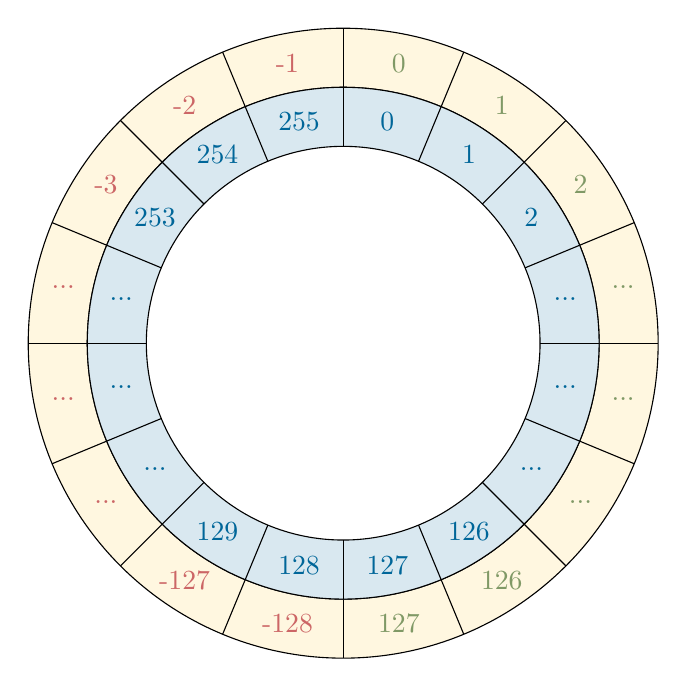
\begin{tikzpicture}[scale=.5]
		\def\RayonListe{6.5}
		\def\EpaisseurListe{1.5}
		\def\LongueurListe{16}
		\draw[fill = UGLiOrange!15] (0,0) circle(\RayonListe+\EpaisseurListe);
		\draw[fill = white] (0,0) circle(\RayonListe);

		\foreach \compt in {0,1,...,\numexpr\LongueurListe-1}
		{\draw (90-\compt/\LongueurListe*360:\RayonListe)--(90-\compt/\LongueurListe*360:\RayonListe+\EpaisseurListe);}

		\foreach \compt in {0,1,2}	{\draw (90-\compt/\LongueurListe*360-180/\LongueurListe:\RayonListe+\EpaisseurListe/2)node{\color{UGLiGreen}\compt};}
		\foreach \compt in {3,4,5}	{\draw (90-\compt/\LongueurListe*360-180/\LongueurListe:\RayonListe+\EpaisseurListe/2)node{\color{UGLiGreen}...};}
		\def \compt{6}	{\draw (90-\compt/\LongueurListe*360-180/\LongueurListe:\RayonListe+\EpaisseurListe/2)node{\color{UGLiGreen} 126};}
		\def \compt{7}	{\draw (90-\compt/\LongueurListe*360-180/\LongueurListe:\RayonListe+\EpaisseurListe/2)node{ \color{UGLiGreen} 127};}
		\def \compt{8}	{\draw (90-\compt/\LongueurListe*360-180/\LongueurListe:\RayonListe+\EpaisseurListe/2)node{\color{UGLiRed} -128};}
		\def \compt{9}	{\draw (90-\compt/\LongueurListe*360-180/\LongueurListe:\RayonListe+\EpaisseurListe/2)node{ \color{UGLiRed} -127};}

		\foreach \compt in {10,11,12}	{\draw (90-\compt/\LongueurListe*360-180/\LongueurListe:\RayonListe+\EpaisseurListe/2)node{\color{UGLiRed}...};}
		\def \compt{13}	{\draw (90-\compt/\LongueurListe*360-180/\LongueurListe:\RayonListe+\EpaisseurListe/2)node{\color{UGLiRed} -3};}
		\def \compt{14}	{\draw (90-\compt/\LongueurListe*360-180/\LongueurListe:\RayonListe+\EpaisseurListe/2)node{\color{UGLiRed} -2};}
		\def \compt{15}	{\draw (90-\compt/\LongueurListe*360-180/\LongueurListe:\RayonListe+\EpaisseurListe/2)node{\color{UGLiRed} -1};}



		\def\RayonListe{5}
		\def\EpaisseurListe{1.5}
		\def\LongueurListe{16}
		\draw[fill=UGLiBlue!15] (0,0) circle(\RayonListe+\EpaisseurListe);
		\draw[fill=white] (0,0) circle(\RayonListe);
		\foreach \compt in {0,1,...,\numexpr\LongueurListe-1}
		{\draw (90-\compt/\LongueurListe*360:\RayonListe)--(90-\compt/\LongueurListe*360:\RayonListe+\EpaisseurListe);}

		\foreach \compt in {0,1,2}	{\draw (90-\compt/\LongueurListe*360-180/\LongueurListe:\RayonListe+\EpaisseurListe/2)node{\color{UGLiBlue}\compt};}
		\foreach \compt in {3,4,5}	{\draw (90-\compt/\LongueurListe*360-180/\LongueurListe:\RayonListe+\EpaisseurListe/2)node{\color{UGLiBlue}...};}
		\def \compt{6}	{\draw (90-\compt/\LongueurListe*360-180/\LongueurListe:\RayonListe+\EpaisseurListe/2)node{\color{UGLiBlue} 126};}
		\def \compt{7}	{\draw (90-\compt/\LongueurListe*360-180/\LongueurListe:\RayonListe+\EpaisseurListe/2)node{\color{UGLiBlue}  127};}
		\def \compt{8}	{\draw (90-\compt/\LongueurListe*360-180/\LongueurListe:\RayonListe+\EpaisseurListe/2)node{\color{UGLiBlue}128};}
		\def \compt{9}	{\draw (90-\compt/\LongueurListe*360-180/\LongueurListe:\RayonListe+\EpaisseurListe/2)node{\color{UGLiBlue} 129};}

		\foreach \compt in {10,11,12}	{\draw (90-\compt/\LongueurListe*360-180/\LongueurListe:\RayonListe+\EpaisseurListe/2)node{\color{UGLiBlue}...};}
		\def \compt{13}	{\draw (90-\compt/\LongueurListe*360-180/\LongueurListe:\RayonListe+\EpaisseurListe/2)node{\color{UGLiBlue} 253};}
		\def \compt{14}	{\draw (90-\compt/\LongueurListe*360-180/\LongueurListe:\RayonListe+\EpaisseurListe/2)node{\color{UGLiBlue} 254};}
		\def \compt{15}	{\draw (90-\compt/\LongueurListe*360-180/\LongueurListe:\RayonListe+\EpaisseurListe/2)node{\color{UGLiBlue} 255};}
	\end{tikzpicture}
\end{center}

\end{document}






